\chapter{Intérêt de la classification spectrale.}

Il existe une très large bibliographie sur la classification non supervisée. Néanmoins, comme le montre la figure suivante, certaines données bien que étant facilement classifiable "à l'œil nu", un algorithme du K-means ne parvient pas à aboutir au résultat escompté.


\begin{figure}[H]
\centering
    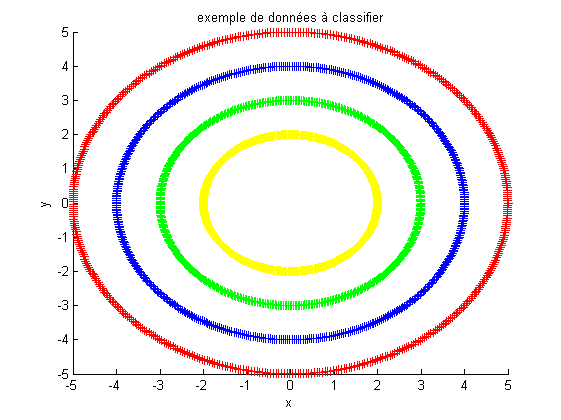
\includegraphics[scale=0.6,angle=0]{Images/DataSet.png}
    \caption{Ensemble de données de départ. Les données sont générer sur un cercle dont le rayon varie selon la classe}
    \label{fig:DataSet}
\end{figure}

\begin{figure}[H]
\centering
    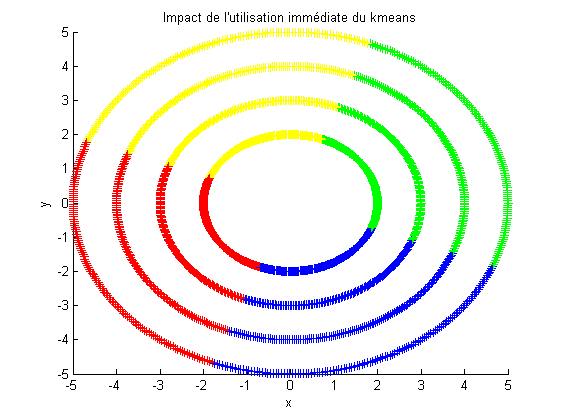
\includegraphics[scale=0.6,angle=0]{Images/AlgoKmeans.png}
    \caption{Application du Kmeans sur cet ensemble de données. Les données ne sont pas correctement classifiées.}
    \label{fig:AlgoKmeans}
\end{figure}

Dans notre cas d'étude, nous devons étudier des signaux temporels dont on ne connait a priori aucunes informations discriminantes. Il est donc nécessaire de parvenir à trouver des paramètres sur lesquelles la classification puisse s'appuyer. L'idée de la classification spectrale va justement d'extraire les valeurs et vecteurs propres d'une certaine matrice afin de classifier les données. Pour ce faire, la classification spectrale propose de créer un graphe à partir des données et d'extraire les informations pertinentes de la matrice de voisinage.

\chapter{Rappel sur la théorie des graphes.}

\section{Définitions de base.}

Un graphe est constitué du couple (V,E,W), où V correspond à ensemble des nœuds du graphe, E correspond à l'ensemble des couple $(v_i,v_j)$ symbolisant le lien entre deux nœuds et W correspond à la matrice de voisinage. Par définition, le coefficient $W_{ij}$ prend comme valeur le poids liant le nœud $v_i$ au nœud $v_j$. Il s'en suit que la matrice W est symétrique. Nous verrons plus tard comment nous pouvons construire une tel matrice.


Par la suite, nous définissons la matrice D, diagonale, qui contient les degrés des nœuds du graphe. Le degré d'un nœud est défini par $d_i = \Sigma_{v_j \in V} W_{ij}$. 
\section{Choix du laplacien de la matrice.}

Il existe trois définition différentes de laplacien d'une matrice. Si on appelle $D$ la matrice de degré du graphe et $W$ la matrice de voisinage du graphe, on aboutie aux définitions suivantes.

\paragraph{Matrice Laplacienne standard non normalisée}

\medskip 

Ce laplacien est donné par la relation:

\begin{equation}
L = D-W
\end{equation}


\paragraph{Matrice Laplacienne normalisée non symétrique}

\medskip 

Ce laplacien est donné par la relation:

\begin{equation}
L = I-D^{-1}W
\end{equation}


\paragraph{Matrice Laplacienne normalisée symétrique}

\medskip 

Ce laplacien est donné par la relation:

\begin{equation}
L = I-D^{-1/2}WD^{-1/2}
\end{equation}

Ces trois matrices présentent les mêmes propriétés:

\begin{itemize}
\item Ces matrices présentent la valeur propres 0 une seule fois pour le vecteur propre $I$ ou $D^{1/2}I$.
\item Ces matrices sont réelles semi-définies positives.
\end{itemize}

Par conséquent, quand nous chercherons à trouver les k plus petites valeurs propres de cette matrice, il nous sera possible très facilement de les récupérer.

\chapter{Construction de la matrice de voisinage.}


Il y a trois choix à faire pour définir la matrice de voisinage d'un graphe.

\section{Choix du type de voisinage.}

Pour un ensemble de nœud donné, il y a plusieurs manière de créer les liens qui vont compléter l'ensemble (E,V,W).

\medskip

\textbf{Graphe des epsilons voisin}: On considère ici que deux nœuds ont un lien si la distance entre eux est inférieur à $\epsilon$.

\medskip

\textbf{Graphe des k-plus proche voisins}: On considère ici que tous les nœuds ont k voisins et qu'ils sont les k-plus proche du nœud considéré.

\medskip

\textbf{Graphe entièrement connecté}: On considère que tous les sommets sont reliés entre eux. 

\medskip

Ici, nous avons implémenté le graphe entièrement connecté car il nous donne de très bons résultats et qu'il est très simple à mettre en place.

\section{Choix de la distance et de la similitude.}

Dans la littérature de la classification, il est nécessaire de choisir une distance et une fonction de similarité.

\medskip

Plusieurs choix s'offre à nous pour les distances:

\begin{itemize}

\medskip

\item \textbf{Distance de Manhattan} : $\Sigma_i|x_i-y_i|$

\medskip

\item \textbf{Distance d'euclidienne} : $(\Sigma_i(x_i-y_i)^2)^(1/2)$

\medskip

\item \textbf{Distance de Minkowski} : $(\Sigma_i|x_i-y_i|^p)^(1/p)$

\medskip

\end{itemize}

La distance euclidienne a ici été choisie.

\medskip

La fonction de similitude doit être une fonction qui va associer une valeur comprise entre 0 et 1 à deux sommet du graphe:

\begin{equation}
f(x_i,x_j) \Rightarrow [0 ; 1]
\end{equation}

La littérature donne plusieurs types de fonction de similitude mais deux sont à retenir.
\begin{itemize}

\item La similitude euclidienne qui est définie par la fonction \\
\begin{equation}
f(x_i,x_j) = \frac{1}{1+\frac{d^2(x_i,x_j)}{\sigma^2}}
\end{equation}

\item La similitude gaussienne qui est définie par la fonction \\
\begin{equation}
f(x_i,x_j) = exp(-\frac{d^2(x_i,x_j)}{2\sigma^2})
\end{equation}

\end{itemize}


Dans les deux cas, le coefficient $\sigma$ est un paramètre qui traduit la dispersion des données. Nous avons ici choisi la similitude gaussienne car elle permet de traduire de manière plus efficace la similitude des données.
 
\section{Choix du paramètre de dispersion.}

Le gros problème pour les données que nous aurons à traiter est que le paramètre $\sigma$ devra être déterminé de manière automatique en fonction des données d'entrées.Ce paramètre va traduire la similitude ou non des différents éléments entre eux et donc va conditionner tous les résultats de l'algorithme.

\medskip

Pour ce faire, une solution assez élégante a été proposée \cite{zelnik2004self} et consiste à définir le paramètre $\sigma$ comme le produit $\sigma_i\sigma_j$, où ces deux coefficient dépendent du voisinage de chaque point.

\medskip

Ainsi, on définit le coefficient par $\sigma_i = d(x_i,x_r)$ où $x_r$ correspond au r-ième voisin le pus proche de $x_i$. Aussi étrange que cela puisse être, après beaucoup de test, on constate comme dans le document \cite{tartare2014contribution} que les meilleurs résultats sont obtenus pour $r=7$ ou $r=9$.

\section*{Conclusion}

Au final, nous arrivons au matrices d'affinité suivante. Les données qui ont été utilisées sont issues d'une IRMs.

\begin{figure}[H]
\centering
    \includegraphics[scale=0.45,angle=0]{Images/MatrixAffinity2.png}
    \caption{Exemple de matrice de similitude.}
    \label{fig:MatrixAffinity2}
\end{figure}


\begin{figure}[H]
\centering
    \includegraphics[scale=0.45,angle=0]{Images/MatrixAffinity.png}
    \caption{Matrice de similitude après utilisation de l'algorithme de classification spectrale.}
    \label{fig:MatrixAffinity}
\end{figure}


\chapter{Quels algorithmes de classification spectrale?}


Les algorithmes de classification spectrale sont répartis en deux classes:

\begin{itemize}
\item La première classe qui va faire une séparation en deux groupes de manière récursive à partir de la seconde plus petite valeur propre de la matrice laplacienne issue du graphe jusqu'à avoir k clusters.
\item La seconde consiste à faire une classification sur les k plus petits vecteurs propres de la matrice laplacienne issue du graphe grâce à un algorithme plus simple comme le K-means.
\end{itemize}

\medskip


Dans le cadre de ce projet, nous avons principalement étudié la seconde classe d'algorithme de classification et particulièrement celui développé par Jordan and Weiss. Au total, nous avons implémenté 4 algorithmes différents de classification spectrale. Les détails théoriques de ces algorithmes peuvent être trouver dans ces références \cite{von2007tutorial} et \cite{shi2000normalized}.

\medskip

Les trois algorithmes correspondent à la seconde classe d'algorithme:

\begin{algorithm}[H]
  \caption{Unnormalized spectral clustering }
  
  \textbf{Inputs}% Inputs section
  \begin{algorithmic}[1]
    \STATE Matrice $W$ matrice de voisinage
    \STATE Entier $k$ nombre de classe
  \end{algorithmic}
  \bigskip

  \textbf{Output}% Output section
  \begin{algorithmic}[1]
    \STATE Vecteur $Ver$ table de vérité calculée.
  \end{algorithmic}
  \bigskip
  
  \textbf{Algorithm}
  \begin{algorithmic}[1]
		\STATE $L\gets$ Laplacien standard de la matrice $W$
     	\STATE $VectP\gets$ matrice contenant les vecteurs propres des k plus petites valeurs propres non nulles de L
     	\STATE $Ver\gets$ résultat de l'algorithme du Kmeans sur la matrice VectP en k clusters.	
  \RETURN $Ver$
  \end{algorithmic}
\end{algorithm}



\begin{algorithm}[H]
  \caption{Normalized spectral clustering, Shi and Malik }
  
  \textbf{Inputs}% Inputs section
  \begin{algorithmic}[1]
    \STATE Matrice $W$ matrice de voisinage
    \STATE Entier $k$ nombre de classe
  \end{algorithmic}
  \bigskip

  \textbf{Output}% Output section
  \begin{algorithmic}[1]
    \STATE Vecteur $Ver$ table de vérité calculée.
  \end{algorithmic}
  \bigskip
  
  \textbf{Algorithm}
  \begin{algorithmic}[1]
		\STATE $L\gets$ Laplacien asymétrique de la matrice $W$
     	\STATE $VectP\gets$ matrice contenant les vecteurs propres des k plus petites valeurs propres non nulles de L
     	\STATE $Ver\gets$ résultat de l'algorithme du Kmeans sur la matrice VectP en k clusters.	
  \RETURN $Ver$
  \end{algorithmic}
\end{algorithm}




\begin{algorithm}[H]
  \caption{Normalized spectral clustering, Jordan and Weiss }
  
  \textbf{Inputs}% Inputs section
  \begin{algorithmic}[1]
    \STATE Matrice $W$ matrice de voisinage
    \STATE Entier $k$ nombre de classe
  \end{algorithmic}
  \bigskip

  \textbf{Output}% Output section
  \begin{algorithmic}[1]
    \STATE Vecteur $Ver$ table de vérité calculée.
  \end{algorithmic}
  \bigskip
  
  \textbf{Algorithm}
  \begin{algorithmic}[1]
		\STATE $L\gets$ Laplacien symétrique de la matrice $W$
     	\STATE $VectP\gets$ matrice contenant les vecteurs propres des k plus petites valeurs propres non nulles de L
     	\STATE normaliser toutes les lignes de la matrice $VectP$
     	\STATE $Ver\gets$ résultat de l'algorithme du Kmeans sur la matrice VectP en k clusters.	
  \RETURN $Ver$
  \end{algorithmic}
\end{algorithm}

\medskip

Le dernier algorithme appartient à la première classe d'algorithme.

\medskip

\begin{algorithm}[H]
  \caption{Normalized spectral recursive clustering, Shi and Malik }
  
  \textbf{Inputs}% Inputs section
  \begin{algorithmic}[1]
    \STATE Matrice $W$ matrice de voisinage
    \STATE Entier $k$ nombre de classe
  \end{algorithmic}
  \bigskip

  \textbf{Output}% Output section
  \begin{algorithmic}[1]
    \STATE Vecteur $Ver$ table de vérité calculée.
  \end{algorithmic}
  \bigskip
  
  \textbf{Algorithm}
  \begin{algorithmic}[1]
		\STATE $L\gets$ Laplacien asymétrique de la matrice $W$
     	\STATE $VectP\gets$ seconde plus petite valeur propre de L
     	\STATE Partititionner le graphe en deux sous-ensemble selon les valeurs de $VectP$
     	\STATE Répéter l'algorithme jusqu'à avoir k clusters.
     	\STATE $Ver\gets$ résultat de l'algorithme.	
  \RETURN $Ver$
  \end{algorithmic}
\end{algorithm}


\chapter{Résultats de l'algorithme et interprétations.}


Nous avons implémenté les différents algorithmes que nous avons précédemment présenté et voici les différents rsultats sur l'ensemble de données que nous avons utilisé dans le chapitre 4.

\begin{figure}[H]
\centering
    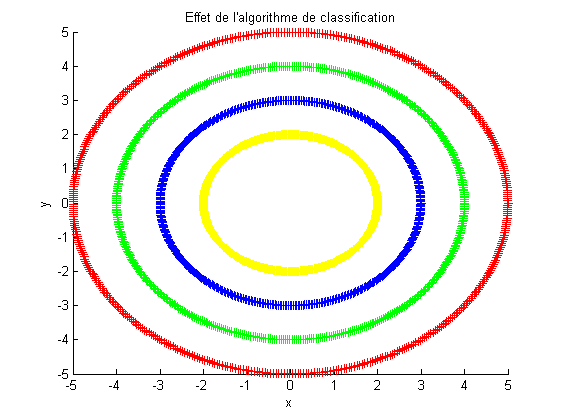
\includegraphics[scale=0.6,angle=0]{Images/AlgoClssification.png}
    \caption{Application du premier algorithme sur les premières données. Les données sont correctement classifiées.}
    \label{fig:AlgoClssification}
\end{figure}

On peut voir que le résultat obtenu est bien celui espéré et que c'est une solution parfaitement viable pour agréger des données dans des clusters bien que les liens entre elles ne soient pas identifiable immédiatement. Les valeurs propres extraites du laplacien et qui sont utilisées pour la classification sont données ci-dessous.

\begin{figure}[H]
\centering
    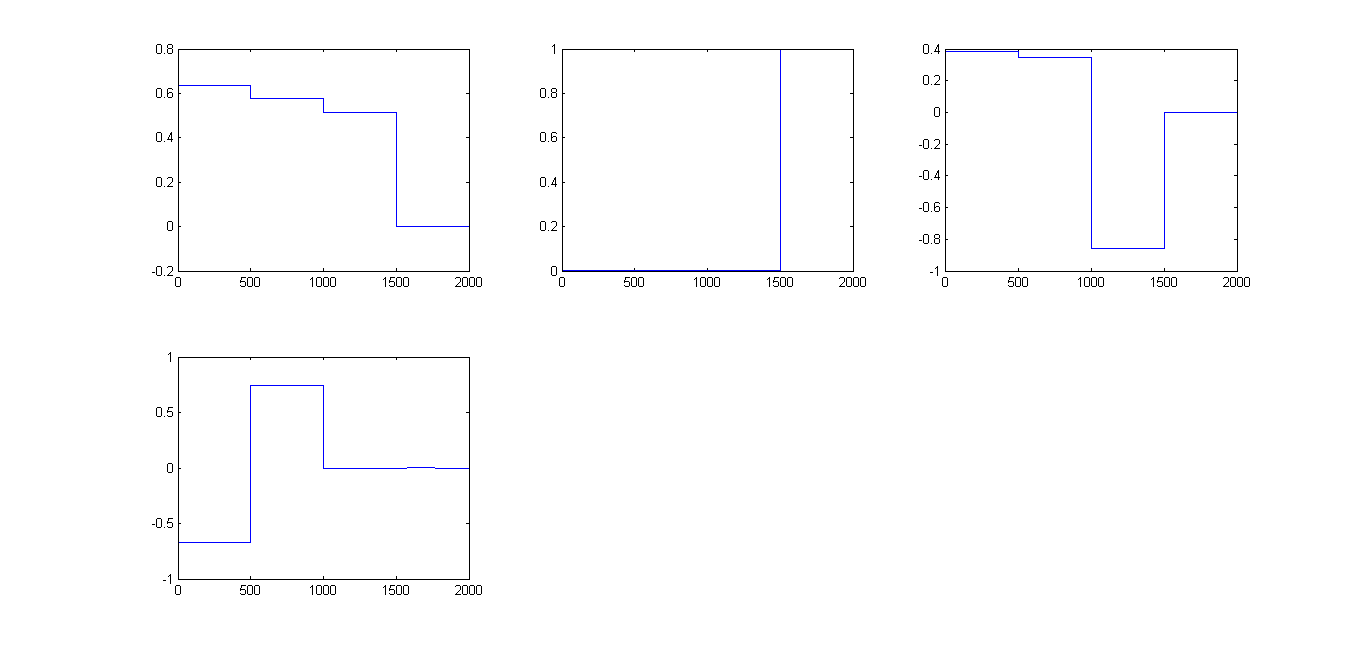
\includegraphics[scale=0.4,angle=0]{Images/VecteursPropres.png}
    \caption{Vecteurs propres extraits du laplacien.}
    \label{fig:VecteursPropres}
\end{figure}

On peut clairement voir comment les K-means sur ces données extraites permettent des discriminer les quatre classes. Nous l'avons testé sur un ensemble de test et les figures suivantes montrent les résultats que nous avons obtenu.


\begin{figure}[H]
\centering
    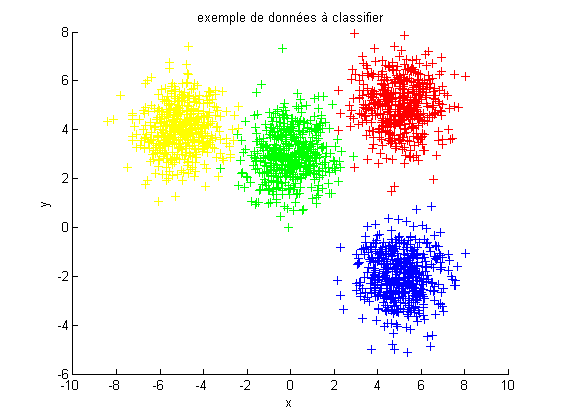
\includegraphics[scale=0.6,angle=0]{Images/DataSet2.png}
    \caption{Second ensemble de données.}
    \label{fig:DataSet2}
\end{figure}

\begin{figure}[H]
\centering
    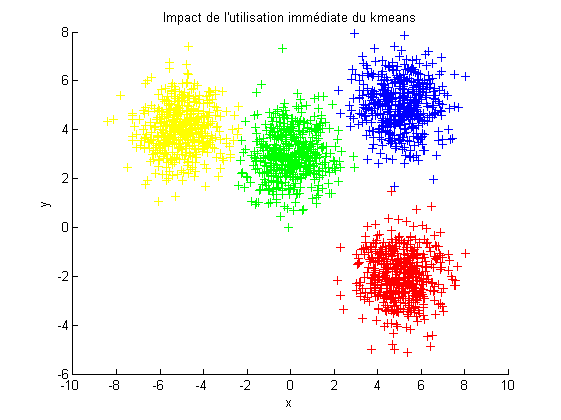
\includegraphics[scale=0.6,angle=0]{Images/AlgoKmeans2.png}
    \caption{Application du Kmeans sur le second ensemble de données.}
    \label{fig:AlgoKmeans2}
\end{figure}

\begin{figure}[H]
\centering
    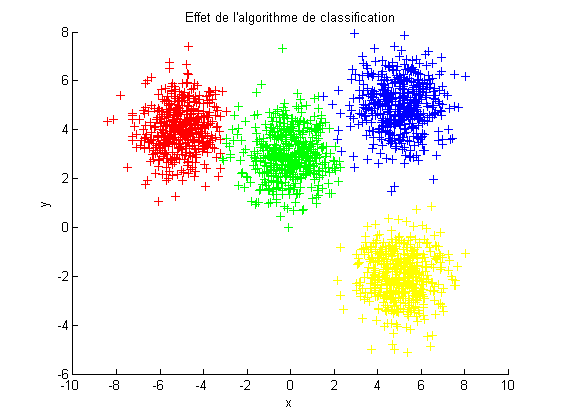
\includegraphics[scale=0.6,angle=0]{Images/AlgoClssification2.png}
    \caption{Application du premier algorithme sur le second ensemble de données.}
    \label{fig:AlgoClssification2}
\end{figure}

\begin{figure}[H]
\centering
    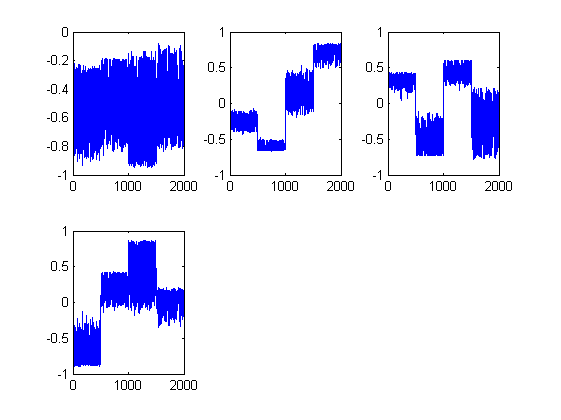
\includegraphics[scale=0.4,angle=0]{Images/VecteursPropres2.png}
    \caption{Vecteurs propres extraits du laplacien.}
    \label{fig:VecteursPropres2}
\end{figure}

Là encore, le résultat est très satisfaisant. Néanmoins, on peut clairement voir que les distributions aléatoires ont un impact sur la régularité des vecteurs propres.


\chapter*{Conclusion}

Au terme de cette étude, nous pouvons extraire ces différents résultats:

\begin{itemize}
\item Tout d'abord, la classification spectrale est particulièrement adaptée pour les problèmes que les algorithmes traditionnels comme le K-means ne peuvent résoudre. On arrive à se placer facilement dans un nouvel espace qui permet d'identifier clairement les éléments appartenant à une même classe.
\item La mise en place des différents algorithme est au final relativement simple et peut couteuse en temps de calcul.
\item Elle est particulièrement adaptée pour le problème que nous étudions.
\end{itemize}

\medskip

Néanmoins, il y a plusieurs contraintes qui faut prendre en compte:

\begin{itemize}
\item Le résultat final est fortement impacté par l'utilisation du K-means à la fin de l'algorithme de classification spectrale. Il arrive que l'algorithme ne converge pas vers les solutions souhaitées en fonction de l'initialisation.
\item Il y a un certain impact du bruit sur les vecteurs propres qui présentent des irrégularités comme le montre la figure \ref{fig:VecteursPropres2}.
\end{itemize}